% ===========================================================================
%  Capitolo 8 — Risultati
%  Lunghezza indicativa: 10–12 pagine. CAPITOLO DI SOLI FATTI.
%
%  Regola: se una frase contiene "perché" o "probabilmente", appartiene al
%  capitolo 9. Qui vanno solo i valori misurati.
%
%  Regola per tutte le tabelle: media ± deviazione standard sui seed. Mai un
%  singolo seed presentato come risultato. Le tabelle per-seed complete vanno
%  nell'appendice C.
% ===========================================================================
\chapter{Risultati}
\label{cap:risultati}

Questo capitolo riporta i valori misurati. Le spiegazioni sono nel
\cref{cap:discussione}: la separazione è mantenuta rigidamente perché rende
verificabile quale parte del lavoro si possa contestare sui dati e quale
sull'argomentazione.

Tutte le tabelle riportano media $\pm$ deviazione standard sui seed. Nessun
singolo seed è presentato come risultato; le tabelle complete per seed sono
nell'\cref{app:tabelle}.

\paragraph{Provenienza dei dati.} \convsegno{}
Le campagne definitive registrano il commit
\code{b91c318ce87e697d7da459cd209a4c11a742fb11} e
\code{dirty=true}: le correzioni di protocollo erano presenti nel working tree.
Gli aggregati sono congelati e controvalidati; il limite di provenienza è
dichiarato nell'\cref{app:inventario}. Le campagne 01--02 usano CPU, la 03 CUDA
per il corpo classico; tutti i circuiti neurali usano PennyLane 0.45.0 con
\code{default.qubit}.

Per l'esperimento~01 la campagna è stata eseguita fra il 31 luglio e il 1 agosto
2026 su CPU, con Python 3.12.9, PyTorch 2.12.0, PennyLane 0.45.0 e backend
\code{default.qubit}. I manifest registrano il commit
\code{b91c318ce87e697d7da459cd209a4c11a742fb11} e il flag \code{dirty=true};
l'aggregato completo è congelato con SHA-256
\code{9ccd5fe09422e0947cfadfc089aeca19cb3b7955d62032c13866a3ded8a6839d}.

\section{Risultati per esperimento}
\label{sec:risultati-per-esperimento}

\subsection{Esperimento 01 --- Proiezioni \texorpdfstring{$Q,K,V$}{Q,K,V} quantistiche}

\begin{table}[htbp]
\centering
\caption[Esperimento 01: loss di validation e perplexity]{%
Esperimento~01, preset \code{thesis}, corpus Shakespeare, 10 seed.
Media $\pm$ deviazione standard; differenza quantistico meno classico.}
\label{tab:risultati-01}
\small
\begin{tabular}{@{}l c c r r@{}}
\toprule
\textbf{Variante} & \textbf{Val.\ loss} & $\PPL$ & \textbf{Parametri} & \textbf{Tempo (s)} \\
\midrule
Classica    & $2{,}56014 \pm 0{,}03278$ & $12{,}94382 \pm 0{,}43068$ & 2945 & $13{,}302 \pm 0{,}935$ \\
Quantistica & $2{,}56557 \pm 0{,}02201$ & $13{,}01093 \pm 0{,}28648$ & 3281 & $618{,}461 \pm 30{,}450$ \\
\midrule
Differenza  & $+0{,}00543$ & $+0{,}06711$ & $+336$ & $+605{,}159$ \\
\bottomrule
\end{tabular}
\end{table}

L'IC al 95\% del delta di loss è $[-0{,}01040;+0{,}02126]$; per la perplexity
è $[-0{,}14100;+0{,}27522]$. Il test $t$ appaiato restituisce rispettivamente
$p=0{,}458$ e $p=0{,}484$. La loss unigramma held-out è $3{,}347305$ ed è
superiore alle medie di entrambe le varianti. Il tempo medio per iterazione è
$0{,}00887 \pm 0{,}00062$ s per la variante classica e
$0{,}41231 \pm 0{,}02030$ s per quella quantistica; il rapporto fra i tempi
totali medi è $46{,}49\times$. Le curve di validation sono nella
\cref{fig:curve-01}.

\begin{figure}[htbp]
  \centering
  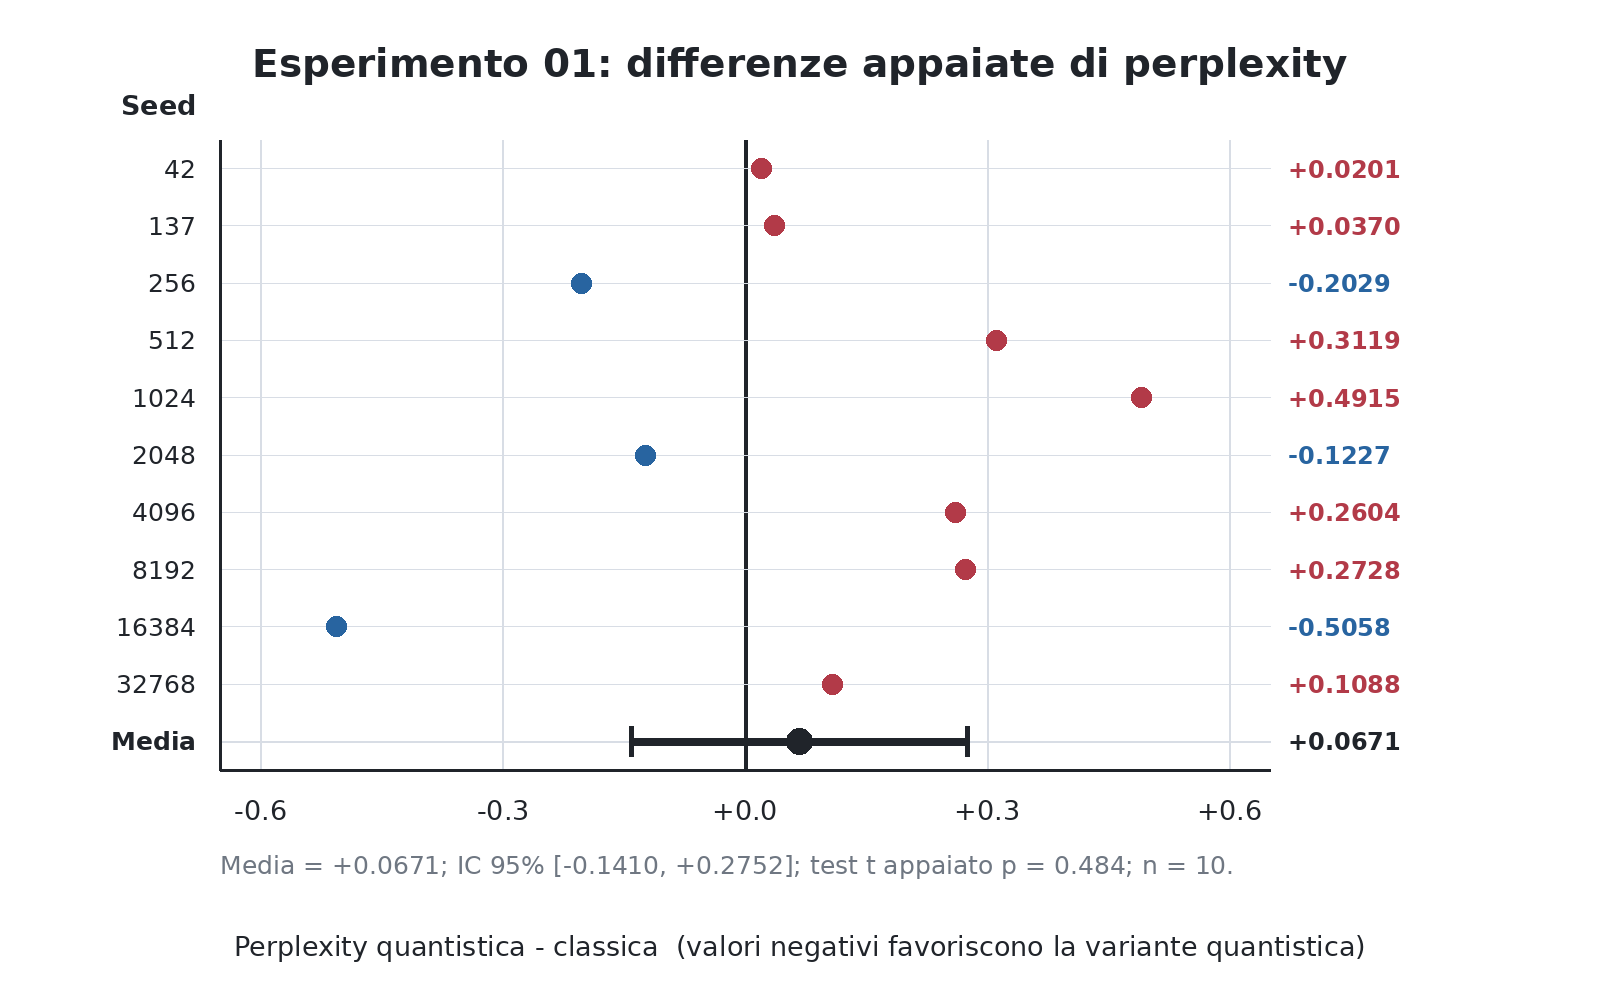
\includegraphics[width=.72\textwidth]{figure/experiment_01_paired_effects.png}
  \caption[Esperimento 01: differenze appaiate]{Differenza di perplexity
  quantistico meno classico per seed. Il punto finale è la media e la barra il
  relativo IC al 95\%.}
  \label{fig:paired-01}
\end{figure}

\subsection{Esperimento 02 --- \emph{Patch embedding} quantistico}

\begin{table}[htbp]
\centering
\caption[Esperimento 02: metriche di classificazione]{%
Esperimento~02, per dataset, 5 seed. Media $\pm$ deviazione standard.
\convsegno}
\label{tab:risultati-02}
\small
\begin{tabular}{@{}l l c c c c r@{}}
\toprule
\textbf{Dataset} & \textbf{Variante} & \textbf{Test acc.} & \textbf{macro-AUC} & \textbf{macro-F1} & $\gap$ & \textbf{Tempo (s)} \\
\midrule
\multirow{2}{*}{PathMNIST} & Classica    & $0{,}72232\pm0{,}02362$ & $0{,}95536\pm0{,}00436$ & $0{,}64840\pm0{,}03101$ & $0{,}01550\pm0{,}01710$ & $1124{,}5\pm38{,}1$ \\
                           & Quantistica & $0{,}69818\pm0{,}01830$ & $0{,}94520\pm0{,}00681$ & $0{,}63598\pm0{,}01843$ & $0{,}03384\pm0{,}02585$ & $10445{,}7\pm712{,}7$ \\
\bottomrule
\end{tabular}
\end{table}

L'accuracy quantistica meno classica è $-0{,}02414$ (IC $t$ al 95\%
$[-0{,}05432;+0{,}00604]$, $p=0{,}091$). L'IC bootstrap è interamente negativo,
ma la decisione primaria segue l'intervallo $t$. La macro-AUC diminuisce di
$0{,}01016$ (IC $[-0{,}01525;-0{,}00507]$, $p=0{,}005$) ed è inferiore in tutti
i cinque seed. La selezione dei checkpoint finali anziché best-validation non
cambia la conclusione. Le curve di apprendimento sono nella \cref{fig:curve-02}.

\begin{figure}[htbp]
\centering
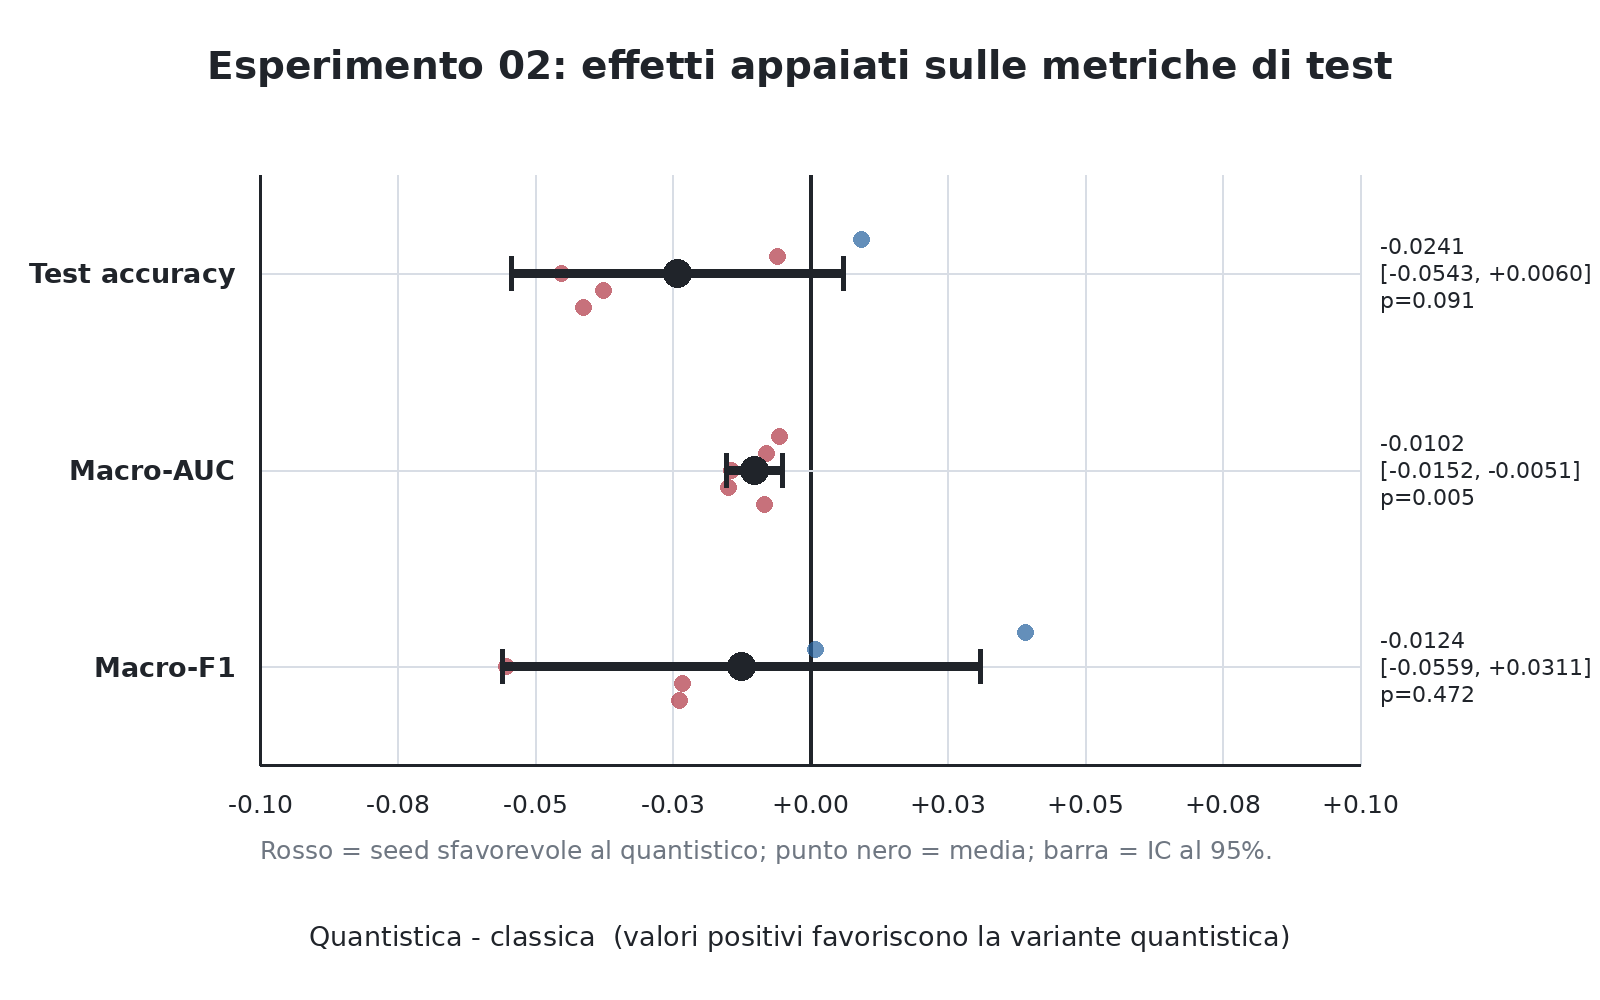
\includegraphics[width=.72\textwidth]{figure/experiment_02_paired_effects.png}
\caption[Esperimento 02: differenze appaiate]{Differenze quantistico meno
classico per le metriche di classificazione; barre: IC al 95\%.}
\label{fig:paired-02}
\end{figure}

\subsection{Esperimento 03 --- Ablazione sulla regolarizzazione}

È la tabella centrale della tesi.

\begin{table}[htbp]
\centering
\caption[Esperimento 03: tabella principale dell'ablazione]{%
Esperimento~03, per dataset e variante, 5 seed. Media $\pm$ deviazione standard.
Il gap $\gap = \acctr - \accte$ è la metrica primaria; $\acctr$ e $\accte$ sono
riportate accanto perché il gap è interpretabile solo a parità di accuracy di
training (\cref{sec:metriche}). \convsegno}
\label{tab:risultati-03}
\scriptsize
\begin{tabular}{@{}l l c c c c c r r@{}}
\toprule
\textbf{Dataset} & \textbf{Variante} & $\acctr$ & $\accte$ & $\gap$ & \textbf{AUC} & \textbf{F1} & \textbf{P.emb.} & \textbf{Tempo (s)} \\
\midrule
\multirow{3}{*}{PathMNIST}
 & \code{vanilla}      & $0{,}806\pm0{,}124$ & $0{,}448\pm0{,}027$ & $0{,}358\pm0{,}141$ & $0{,}768\pm0{,}026$ & $0{,}359\pm0{,}016$ & \num{1480} & $29{,}7\pm1{,}2$ \\
 & \code{bounded\_mlp} & $0{,}886\pm0{,}053$ & $0{,}464\pm0{,}029$ & $0{,}423\pm0{,}050$ & $0{,}754\pm0{,}020$ & $0{,}385\pm0{,}023$ & \num{1880} & $30{,}0\pm1{,}1$ \\
 & \code{quantum\_reg} & $0{,}950\pm0{,}050$ & $0{,}379\pm0{,}066$ & $0{,}571\pm0{,}096$ & $0{,}719\pm0{,}046$ & $0{,}322\pm0{,}055$ & \num{1540} & $1818{,}2\pm129{,}2$ \\
\midrule
\multirow{3}{*}{BloodMNIST}
 & \code{vanilla}      & $0{,}874\pm0{,}067$ & $0{,}565\pm0{,}039$ & $0{,}309\pm0{,}079$ & $0{,}845\pm0{,}027$ & $0{,}472\pm0{,}054$ & \num{1480} & $14{,}9\pm0{,}1$ \\
 & \code{bounded\_mlp} & $0{,}932\pm0{,}029$ & $0{,}536\pm0{,}051$ & $0{,}396\pm0{,}069$ & $0{,}819\pm0{,}035$ & $0{,}449\pm0{,}055$ & \num{1880} & $15{,}2\pm0{,}1$ \\
 & \code{quantum\_reg} & $0{,}916\pm0{,}139$ & $0{,}421\pm0{,}041$ & $0{,}495\pm0{,}157$ & $0{,}739\pm0{,}027$ & $0{,}348\pm0{,}046$ & \num{1540} & $961{,}5\pm26{,}0$ \\
\midrule
\multirow{3}{*}{DermaMNIST}
 & \code{vanilla}      & $0{,}772\pm0{,}104$ & $0{,}634\pm0{,}023$ & $0{,}138\pm0{,}125$ & $0{,}661\pm0{,}039$ & $0{,}158\pm0{,}041$ & \num{1480} & $13{,}8\pm0{,}1$ \\
 & \code{bounded\_mlp} & $0{,}770\pm0{,}105$ & $0{,}650\pm0{,}016$ & $0{,}120\pm0{,}117$ & $0{,}599\pm0{,}096$ & $0{,}159\pm0{,}042$ & \num{1880} & $14{,}0\pm0{,}1$ \\
 & \code{quantum\_reg} & $0{,}832\pm0{,}108$ & $0{,}628\pm0{,}041$ & $0{,}204\pm0{,}140$ & $0{,}607\pm0{,}035$ & $0{,}158\pm0{,}021$ & \num{1540} & $891{,}9\pm5{,}7$ \\
\bottomrule
\end{tabular}
\end{table}

\paragraph{Tracce diagnostiche.}
\begin{table}[htbp]
\centering
\caption[Esperimento 03: diagnostica su gradienti e attivazioni]{%
Norma $L^2$ media del gradiente in uscita da \code{patch\_embed.compression} e
frazione di attivazioni in saturazione (definita dalla \cref{eq:saturazione}),
mediate su epoche e seed. Il modulo osservato è identico nelle tre varianti.}
\label{tab:diagnostica-03}
\small
\begin{tabular}{@{}l c c@{}}
\toprule
\textbf{Variante} & \textbf{Norma media del gradiente} & \textbf{Frazione di saturazione} \\
\midrule
\code{vanilla}      & $0{,}198$ & $0{,}00113$ \\
\code{bounded\_mlp} & $0{,}185$ & $0{,}00049$ \\
\code{quantum\_reg} & $0{,}250$ & $0{,}00453$ \\
\bottomrule
\end{tabular}
\end{table}

Il delta di gap quantistico meno \code{bounded\_mlp} è $+0{,}148$ su
PathMNIST, $+0{,}100$ su BloodMNIST e $+0{,}085$ su DermaMNIST; il segno è
contrario a H3 in 12 blocchi dataset/seed su 15. Saturazione e gradienti non
indicano un collasso banale dell'ottimizzazione.

Il gap medio delle tre varianti, dataset per dataset, è rappresentato nella
\cref{fig:gap-03}.

\begin{figure}[htbp]
\centering
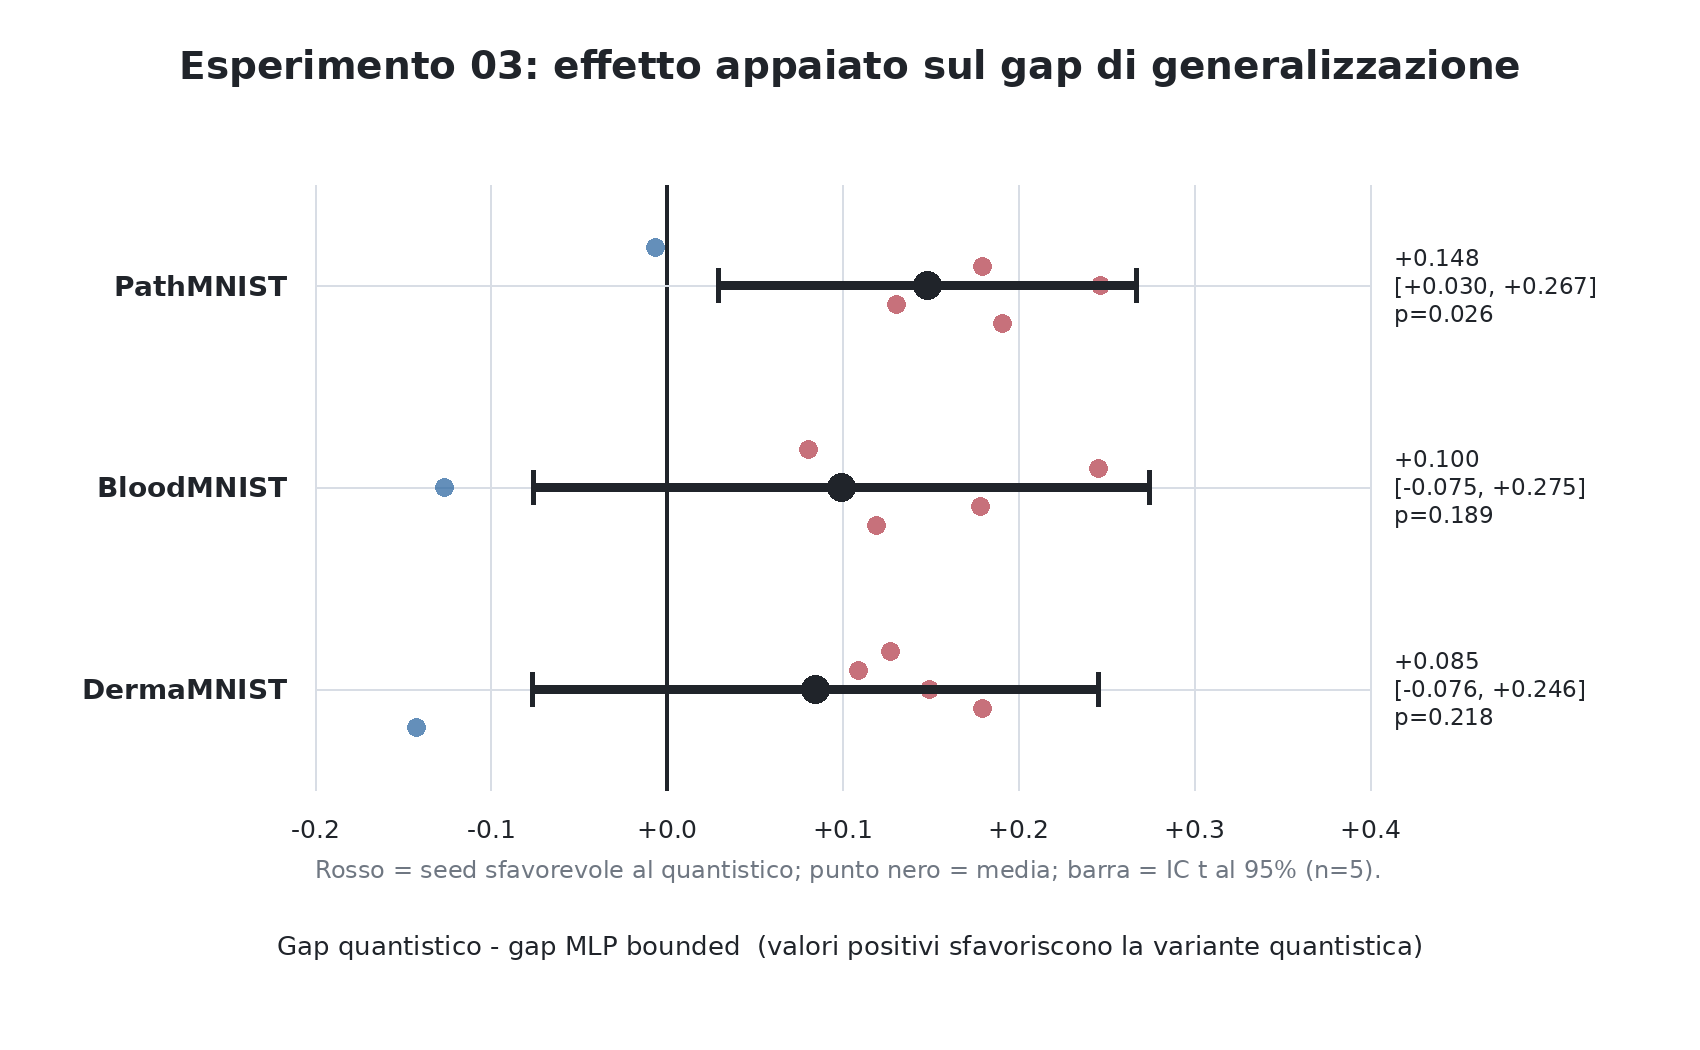
\includegraphics[width=.72\textwidth]{figure/experiment_03_paired_gap_effects.png}
\caption[Esperimento 03: differenze appaiate del gap]{Differenza di gap
\code{quantum\_reg} meno \code{bounded\_mlp} per dataset e seed. Valori
positivi sono contrari all'ipotesi di regolarizzazione; il punto aggregato
riporta media e IC al 95\%.}
\label{fig:paired-gap-03}
\end{figure}

\subsection{Esperimento 04 --- Kernel di fedeltà}

\begin{table}[htbp]
\centering
\caption[Esperimento 04: metriche di separabilità]{%
Esperimento~04, BreastMNIST, 80${+}$20 campioni, PCA a 8 componenti.
Media $\pm$ deviazione standard su 20 ripetizioni. Il criterio di Fisher è
la metrica primaria; il rapporto $\rho$ è descrittivo e non confrontabile fra
scale diverse (\cref{sec:metriche}). \convsegno}
\label{tab:risultati-04}
\small
\begin{tabular}{@{}l c c c c c@{}}
\toprule
\textbf{Kernel} & \code{intra\_0} & \code{intra\_1} & \code{inter} & $\rho$ & $F$ \\
\midrule
Coseno & $0{,}8922 \pm 0{,}0142$ & $0{,}8825 \pm 0{,}0158$ & $0{,}8816 \pm 0{,}0133$ & $1{,}0066 \pm 0{,}0043$ & $0{,}0180 \pm 0{,}0200$ \\
RBF & $0{,}6084 \pm 0{,}0108$ & $0{,}5473 \pm 0{,}0405$ & $0{,}5547 \pm 0{,}0210$ & $1{,}0424 \pm 0{,}0294$ & $0{,}0446 \pm 0{,}0513$ \\
Fedeltà (IQP) & $0{,}0172 \pm 0{,}0038$ & $0{,}0171 \pm 0{,}0067$ & $0{,}0145 \pm 0{,}0028$ & $1{,}1799 \pm 0{,}1451$ & $0{,}0029 \pm 0{,}0032$ \\
\bottomrule
\end{tabular}
\end{table}

Le otto componenti PCA spiegano $0{,}7654 \pm 0{,}0113$ della varianza
(intervallo osservato $[0{,}7459,0{,}7837]$). Sulla metrica primaria, la
differenza IQP meno coseno è $-0{,}01515$; IQP meno RBF è $-0{,}04168$. Il
rapporto $\rho$ ha invece segno opposto, come discusso nella
\cref{sec:limiti-statistici}: non sostituisce la metrica primaria dichiarata.

\begin{figure}[htbp]
\centering
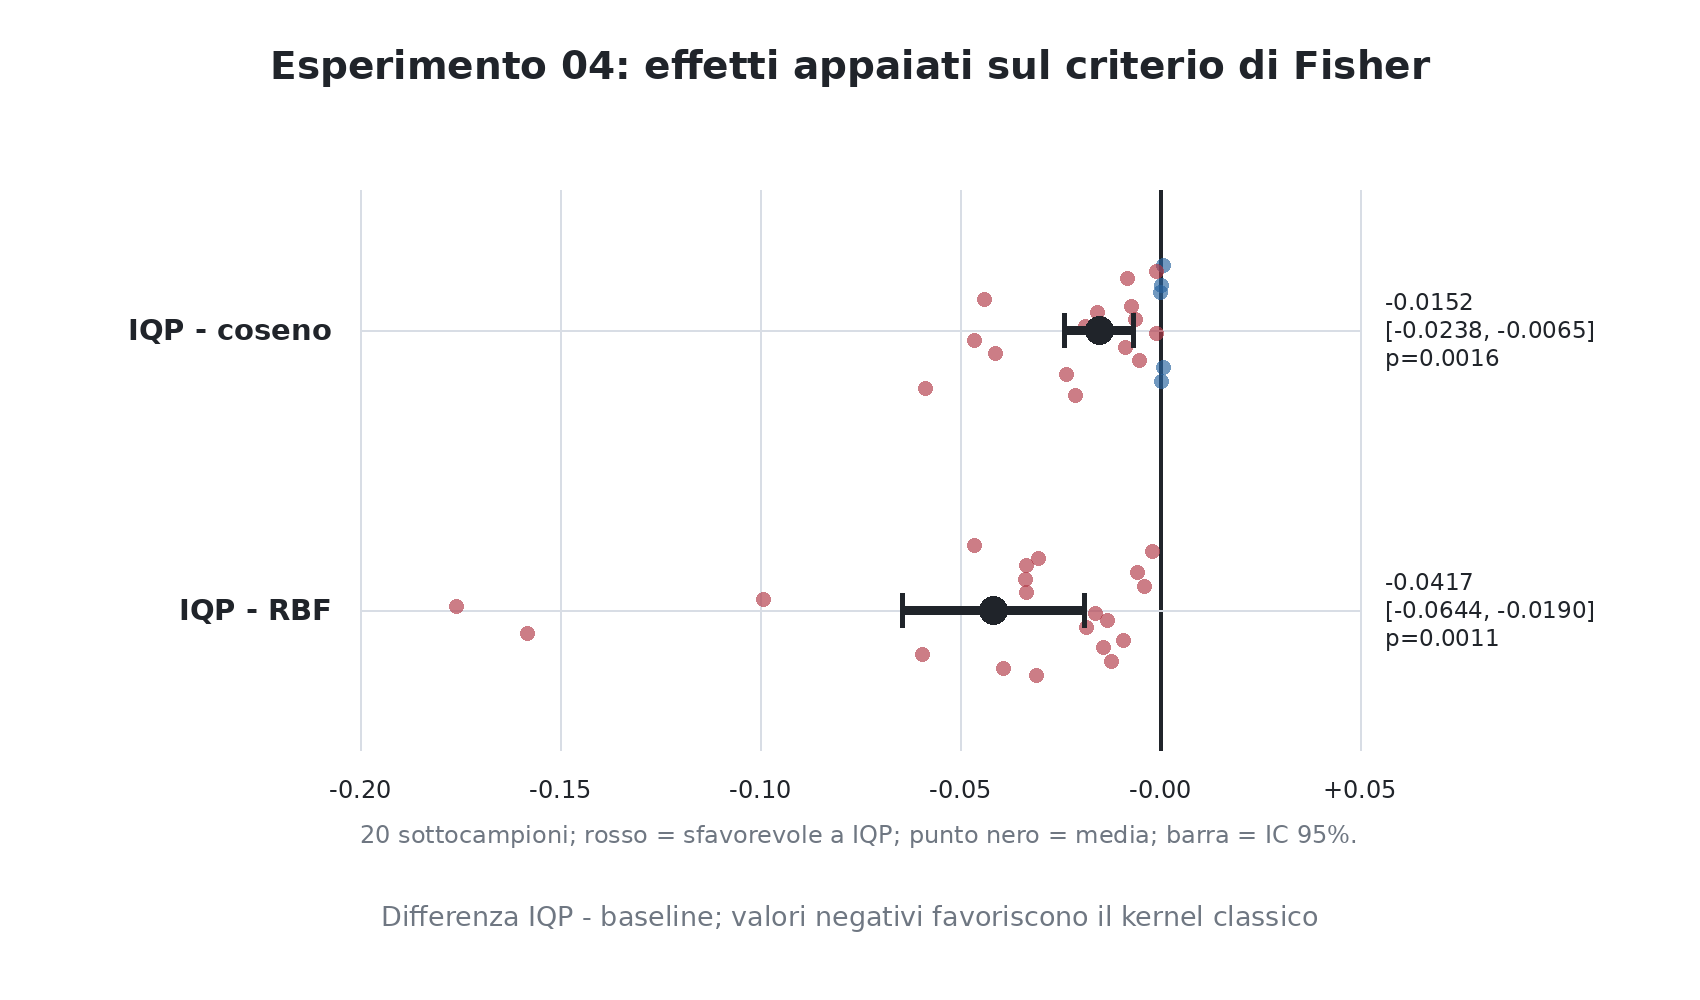
\includegraphics[width=.72\textwidth]{figure/experiment_04_fisher_effects.png}
\caption[Esperimento 04: effetti sul criterio di Fisher]{Differenze appaiate
IQP meno coseno e IQP meno RBF. Valori negativi indicano separabilità inferiore
del kernel quantistico; barre: IC al 95\%.}
\label{fig:fisher-04}
\end{figure}

La validazione predittiva fuori campione, con SVC a kernel precomputato sul test
ufficiale BreastMNIST e $C$ selezionato per cross-validation sui soli dati di
training, va nella stessa direzione della metrica primaria. IQP è inferiore a
coseno e RBF su balanced accuracy, macro-AUC e macro-F1 in tutti e tre i regimi di
composizione: nel regime 80/20 la balanced accuracy è $0{,}511$ contro $0{,}594$
del coseno, nel 50/50 $0{,}607$ contro $0{,}673$ e nel 27/73 $0{,}569$ contro
$0{,}688$. I valori completi sono nell'\cref{tab:validazione-svc-04}.

\begin{figure}[htbp]
\centering
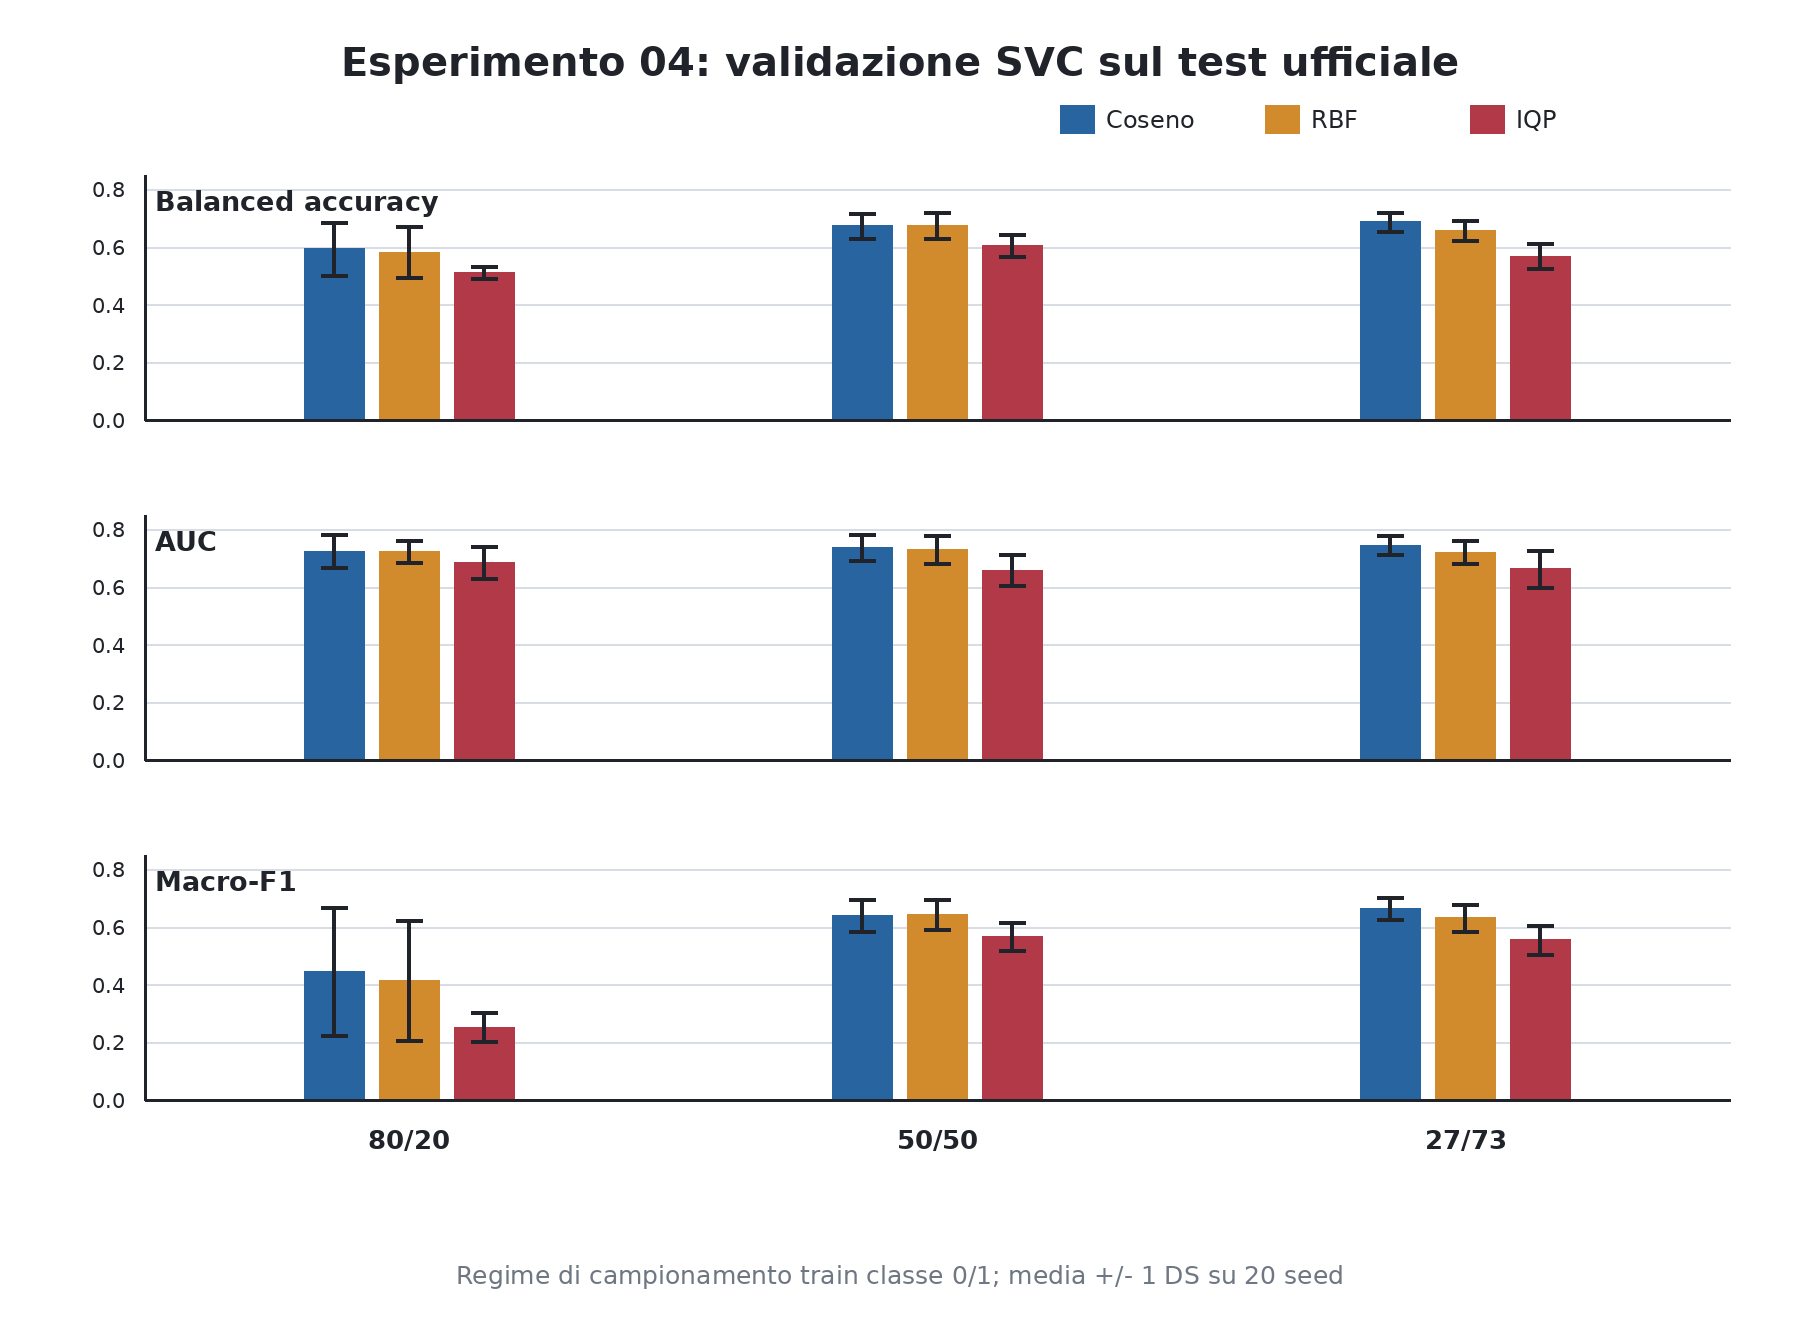
\includegraphics[width=.85\textwidth]{figure/experiment_04_svc_metrics.png}
\caption[Esperimento 04: metriche SVC]{Balanced accuracy, macro-AUC e macro-F1
della SVC con kernel precomputato nei regimi 80/20, 50/50 e 27/73. Le barre
riassumono la variabilità sui venti sottocampioni di training.}
\label{fig:svc-04}
\end{figure}

\section{Differenze appaiate}
\label{sec:differenze-appaiate}

Le differenze dell'esperimento 01 sono riportate nell'\cref{tab:seed-01}; le
figure \cref{fig:paired-01,fig:paired-02,fig:paired-gap-03,fig:fisher-04}
mostrano i punti appaiati, la media e l'intervallo. I valori aggregati sono
riuniti nella \cref{tab:statistica}.

Dove il segno della differenza non è consistente fra i seed, l'incoerenza è
riportata insieme al valore medio, perché descrive la stabilità del confronto.

\section{Intervalli di confidenza e dimensioni dell'effetto}
\label{sec:intervalli}

\begin{table}[htbp]
\centering
\caption[Analisi statistica dei confronti appaiati]{%
Analisi appaiata prodotta da \code{paired\_comparison()} sulle metriche primarie.
Sono riportati insieme differenza media, entrambi gli intervalli di confidenza, i
due valori $p$ e la dimensione dell'effetto: il valore $p$ da solo non è un
risultato (\cref{sec:statistica}). \convsegno}
\label{tab:statistica}
\scriptsize
\begin{tabular}{@{}l l c c c c c c@{}}
\toprule
\textbf{Confronto} & \textbf{Metrica} & $\dmean$ & $\IC$ ($t$) & $\IC$ (boot.) & $p_{t}$ & $p_{W}$ & $\dz$ \\
\midrule
04 IQP--coseno & Fisher & $-0{,}01515$ & $[-0{,}02379;-0{,}00652]$ & $[-0{,}02345;-0{,}00769]$ & $0{,}00161$ & $0{,}000322$ & $-0{,}821$ \\
04 IQP--RBF & Fisher & $-0{,}04168$ & $[-0{,}06438;-0{,}01899]$ & $[-0{,}06452;-0{,}02322]$ & $0{,}00109$ & $1{,}91\times10^{-6}$ & $-0{,}860$ \\
01 QGPT & PPL & $+0{,}06711$ & $[-0{,}14100;+0{,}27522]$ & $[-0{,}11048;+0{,}22839]$ & $0{,}484$ & $0{,}4316$ & $+0{,}231$ \\
02 QViT & Accuracy & $-0{,}02414$ & $[-0{,}05432;+0{,}00604]$ & $[-0{,}04208;-0{,}00386]$ & $0{,}0905$ & $0{,}1875$ & $-0{,}993$ \\
03 PathMNIST & Gap & $+0{,}14838$ & $[+0{,}030;+0{,}267]$ & $[+0{,}070;+0{,}212]$ & $0{,}026$ & $0{,}125$ & $+1{,}550$ \\
03 BloodMNIST & Gap & $+0{,}09954$ & $[-0{,}075;+0{,}275]$ & $[-0{,}024;+0{,}195]$ & $0{,}189$ & $0{,}3125$ & $+0{,}706$ \\
03 DermaMNIST & Gap & $+0{,}08462$ & $[-0{,}076;+0{,}246]$ & $[-0{,}034;+0{,}159]$ & $0{,}218$ & $0{,}3125$ & $+0{,}653$ \\
\bottomrule
\end{tabular}
\end{table}

Gli intervalli distinguono neutralità incerta per H1, stima sfavorevole ma IC
dell'accuracy attraversato da zero per H2, direzione media sfavorevole coerente
fra dataset per H3 e intervalli interamente opposti all'atteso per H4.

L'unica divergenza rilevante fra $t$-test, bootstrap e Wilcoxon riguarda
l'accuracy dell'esperimento 02, dove l'intervallo bootstrap è interamente negativo
mentre quello $t$ attraversa lo zero; la decisione primaria segue l'intervallo
$t$, come stabilito nella \cref{sec:statistica}. La dimensione dell'effetto è
interpretata con le soglie convenzionali di \textcite{cohen1988statistical}
($0{,}2$, $0{,}5$, $0{,}8$), che restano convenzioni, e va letta tenendo presente
il limite di rilevabilità $\dz \ge 1{,}68$ della \cref{ssec:potenza}.

Il conteggio dei parametri per componente e i tempi di esecuzione delle tre
campagne con addestramento sono nell'\cref{app:tabelle}. I rapporti temporali
restano separati per esperimento: una singola figura accuracy--tempo
suggerirebbe una frontiera comune fra workload non omogenei.

\section{Verifica delle ipotesi}
\label{sec:verifica-ipotesi}

\begin{table}[htbp]
\centering
\caption[Esito delle quattro ipotesi]{%
Esito delle quattro ipotesi della \cref{tab:ipotesi}. L'esito
\rifiutataopposta{} indica che l'intervallo di confidenza è interamente
collocato nella direzione contraria a quella attesa. \convsegno}
\label{tab:verifica-ipotesi}
\small
\begin{tabularx}{\textwidth}{@{}c X c c c c@{}}
\toprule
\textbf{\#} & \textbf{Metrica primaria} & $\dmean$ & $\IC$ & $p$ & \textbf{Esito} \\
\midrule
H1 & Perplexity di validation & $+0{,}06711$ & $[-0{,}14100;+0{,}27522]$ & $0{,}484$ & \rifiutata \\
H2 & Test accuracy & $-0{,}02414$ & $[-0{,}05432;+0{,}00604]$ & $0{,}091$ & \rifiutata \\
H3 & Gap (tre dataset) & $+0{,}148;+0{,}100;+0{,}085$ & vedi \cref{tab:statistica} & --- & \rifiutata \\
H4 & Criterio di Fisher & $-0{,}01515$ & $[-0{,}02379;-0{,}00652]$ & $0{,}00161$ & \rifiutataopposta \\
\bottomrule
\end{tabularx}
\end{table}

Dove l'ipotesi non è rifiutata, il dato risulta compatibile con l'assenza di
effetto senza dimostrare un'equivalenza, e l'ampiezza di effetto ancora
compatibile è quella delimitata dall'intervallo di confidenza riportato in
tabella. L'espressione «prestazioni equivalenti» non compare in questa tesi,
perché non sarebbe sostenibile senza una soglia di equivalenza fissata a priori
(\cref{sec:falsificazione}).

Le spiegazioni sono rimandate al \cref{cap:discussione}.
